\documentclass{article}

\usepackage{../handout}
\usepackage{proof}
% Handout Numbers

\newcommand{\PAOneNum}{1}
\newcommand{\WAOneNum}{2}
\newcommand{\PATwoNum}{3}
\newcommand{\PAThreeNum}{4}
\newcommand{\WATwoNum}{5}
\newcommand{\WATwoSolNum}{6}
\newcommand{\WAOneSolNum}{7}
\newcommand{\WAThreeNum}{8}
\newcommand{\WAFourNum}{9}
\newcommand{\WAThreeSolNum}{10}
\newcommand{\PAFourNum}{11}
\newcommand{\WAFourSolNum}{12}
\newcommand{\WAFiveNum}{13}
\newcommand{\WAFiveSolNum}{14}
\newcommand{\WASixNum}{15}
\newcommand{\WASixSolNum}{16}
\newcommand{\PAFiveNum}{17}
\newcommand{\WASevenNum}{18}
\newcommand{\WASevenSolNum}{19}
\newcommand{\PAExtraNum}{20}
\newcommand{\WAEightNum}{21}
\newcommand{\WAEightSolNum}{22}
\newcommand{\PASixNum}{23}
\newcommand{\WANineNum}{24}
\newcommand{\WANineSolNum}{25}
\newcommand{\WATenNum}{26}
\newcommand{\WATenSolNum}{27}
\newcommand{\WAElevenNum}{28}
\newcommand{\WAElevenSolNum}{29}

\usepackage{fullpage}
\usepackage{graphicx}
\usepackage{amssymb}


\newtheorem{theorem}{Theorem}
\newcommand{\thmLabel}[1]{{\rm (}{\em #1\/}{\rm )}}

\newcommand{\ntsym}[1]{\hbox{\em #1}}
\newcommand{\tsym}[1]{\hbox{\rm #1}}
\newcommand{\infertext}[2]{\infer{{\textrm{#1}}}{#2}}

\def\ra{\rightarrow}     % grammar "rewrites-as" symbol
\def\ep{\varepsilon}     % epsilon for empty-string


\begin{document}
\handout{\WATenSolNum}{4}{Solutions to Written Assignment 10}

\begin{enumerate}
\item
\begin{enumerate}
\item It is convenient to first draw a control-flow graph and compute
the live variable sets:

\begin{center}
\hspace*{-10mm}\includegraphics[angle=0,scale=0.95]{wa10-s1a}
\end{center}

The register interference graph is then easy to compute:

\begin{center}
\includegraphics[angle=0]{wa10-s1b}
\end{center}

\item Now we run the register allocation heuristics.  Since we have
only 4 registers, we have to pick some temporary to spill.
Arbitrarily, we choose to spill \texttt{b}. 
Our code becomes: 

\begin{verbatim}
L0: e := 0
    b := 1
    store b
    d := 2
L1: load b
    a := b+2
    c := d+5
    e := e + c
    f := a * a
    if f < c goto L3
L2: e := e + f
    goto L4
L3: e := e + 2
L4: d := d + 4
    load b
    b := b - 4
    store b
    load b /* You might omit this */
    if b != d goto L1
L5:
\end{verbatim}
and the new register interference graph is
\begin{center}
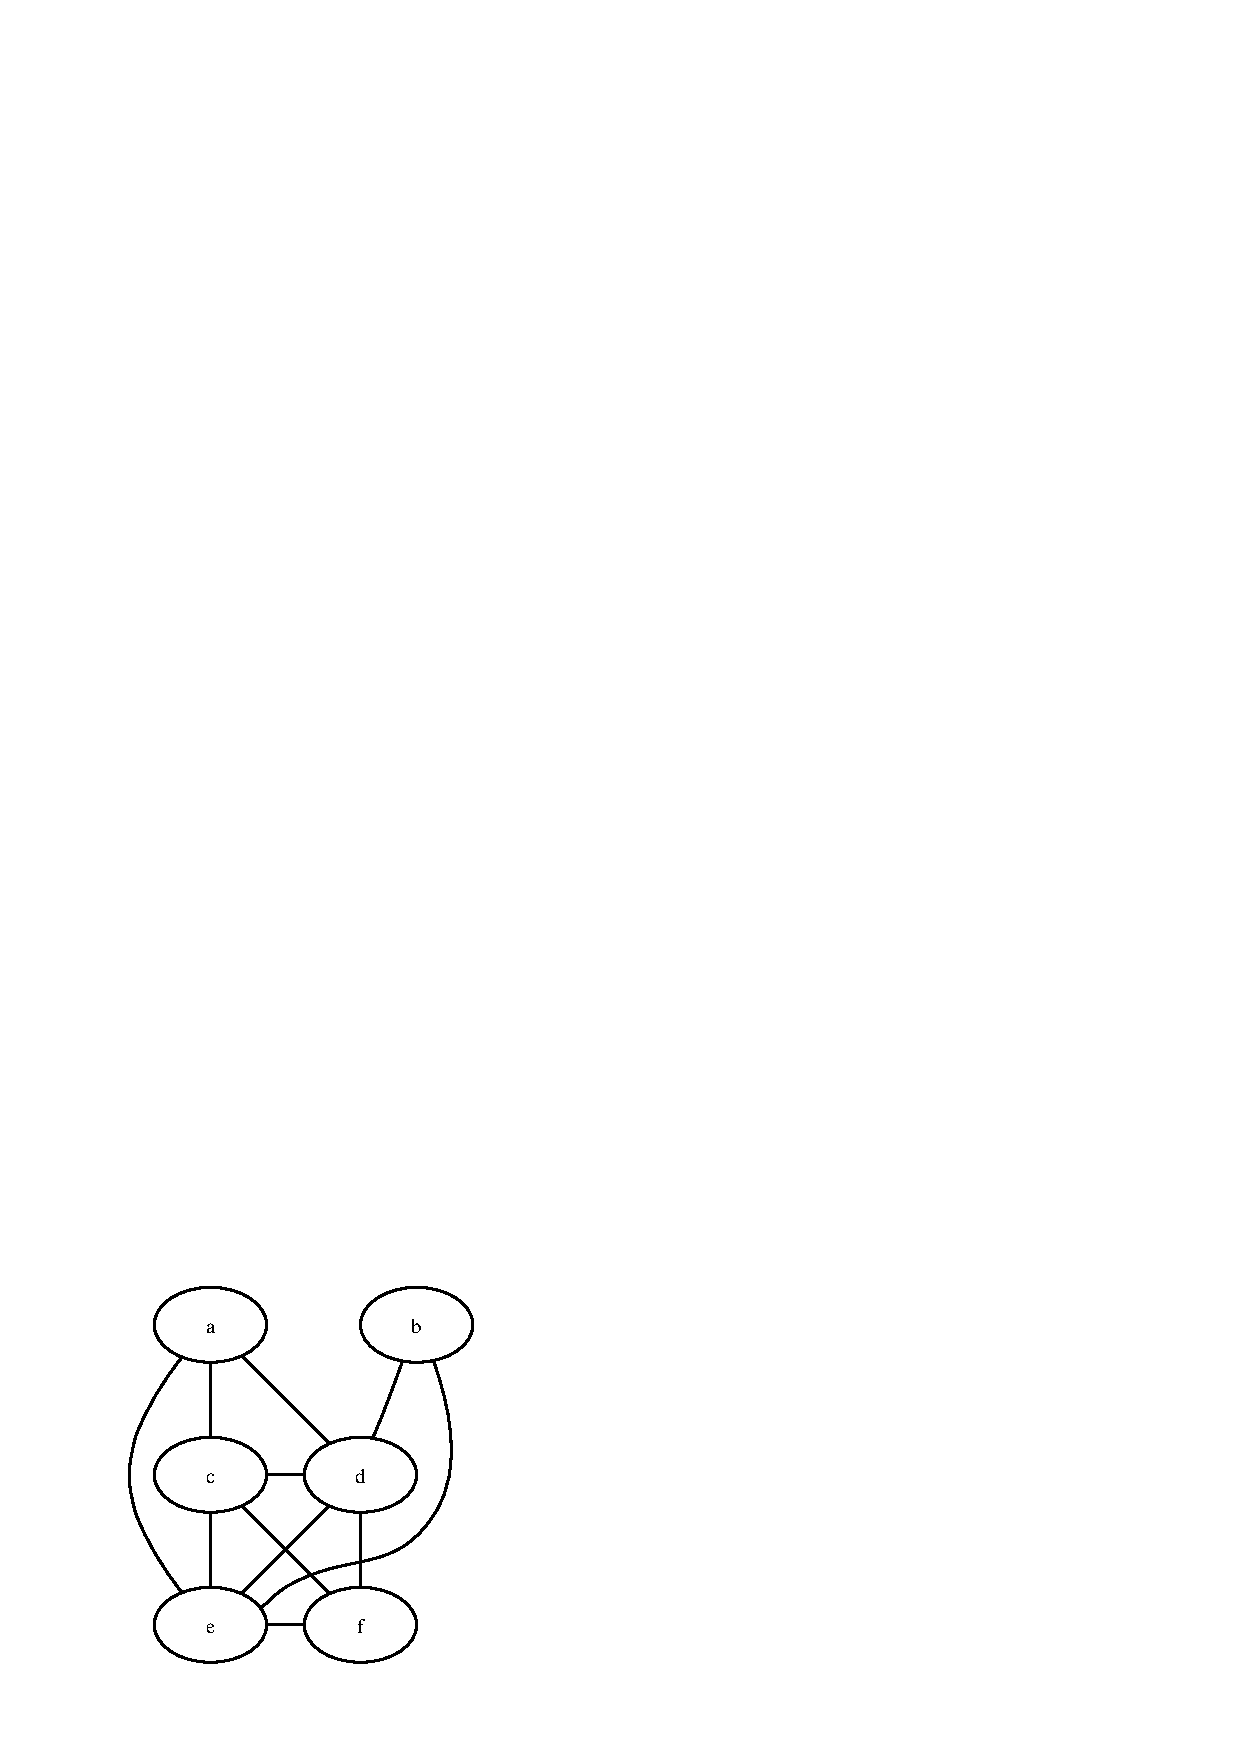
\includegraphics[angle=0]{wa10-s1c}
\end{center}
This can be 4-colored by our register allocation heuristics. 
One possible assignment of registers to
temporaries is \texttt{b} and \texttt{c} to \texttt{r1}, \texttt{d} to
\texttt{r2}, \texttt{e} to \texttt{r3}, and \texttt{a}, \texttt{f} to
\texttt{r4}.

Our code becomes
\begin{verbatim}
L0: r3 := 0
    r1 := 1
    store r1
    r2 := 2
L1: load r1
    r4 := r1+2
    r1 := r2+5
    r3 := r3 + r1
    r4 := r4 * r4
    if r4 < r1 goto L3
L2: r3 := r3 + r4
    goto L4
L3: r3 := r3 + 2
L4: r2 := r2 + 4
    load r1
    r1 := r1 - 4
    store r1
    load r1 /* You might omit this */
    if r1 != r2 goto L1
L5:
\end{verbatim}


\end{enumerate}

\newpage

\item 

\begin{enumerate}
\item 
The instruction scheduling heuristics computes the following instruction
dependence graph. 
\begin{center}
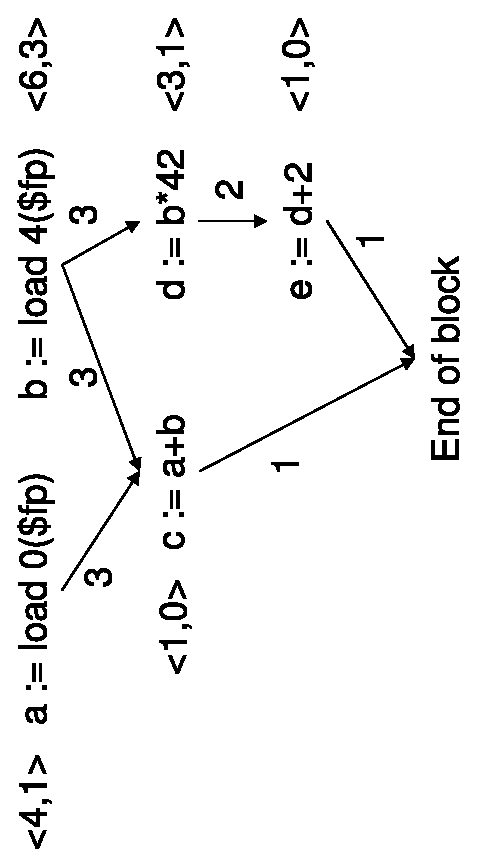
\includegraphics[angle=-90,scale=0.5]{wa10-s2a}
\end{center}
Based on the above graph, the heuristics comes up with the following
schedule. 
\begin{verbatim}
 b := load 4($fp)
 a := load 0($fp)
 nop
 d := b*42
 c := a+b
 e := d+2
\end{verbatim}

\item
Consider the following basic block, along with its instruction
dependence graph. 
\begin{center}
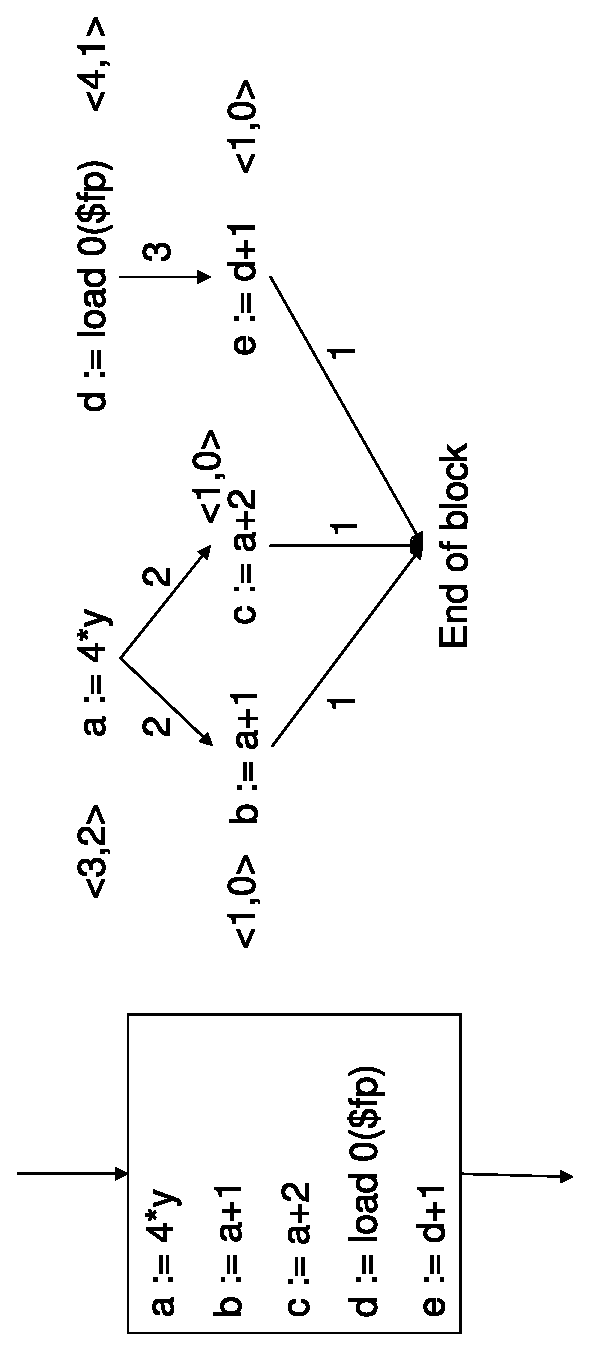
\includegraphics[angle=-90,scale=0.5]{wa10-s2b}
\end{center}
The heuristic comes up with the following schedule, which takes $6$
cycles. 

\begin{verbatim}
 d := load 0($fp)
 a := 4*y
 nop
 b := a+1
 c := a+2
 e := d+1
\end{verbatim}

The optimal schedule is as follows, which takes $5$ cycles. 

\begin{verbatim}
 a := 4*y
 d := load 0($fp)
 b := a+1
 c := a+2
 e := d+1
\end{verbatim}


\item
Consider the following control flow graph. 
\begin{center}
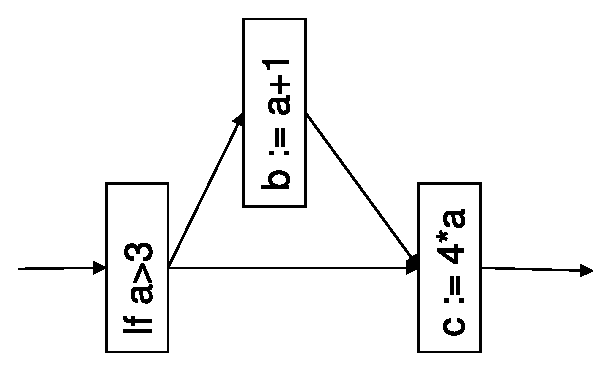
\includegraphics[angle=-90,scale=0.5]{wa10-s2c}
\end{center}

Optimal basic-block scheduling yields the following schedule, which takes $4$
or $5$ cycles (depending on whether the branch evaluates to true or false). 
\begin{verbatim}
    if a>3 jump L1
    *nop 
    b := a+1
L1: c := 4*a
    nop
\end{verbatim}  

The best schedule is as follows, which takes $3$ or $4$ cycles
(depending on whether the branch evaluates to true or false). 
\begin{verbatim}
    c := 4*a
    if a>3 jump L1
    *nop
    b := a+1
L1: 
\end{verbatim}

\end{enumerate}

\item
\begin{enumerate}
\item As-is, this code takes 10 cycles to complete, and if we schedule it
we'll move the multiplication up so that the block takes 9 cycles.
If, however, we first perform register allocation, then \texttt{b} and
\texttt{d} will be stored in the same register, creating a false
dependency and preventing the multiplication instruction from being
moved up by the instruction scheduler.

\item Here is an example of a program for which register allocation
is better done before instruction scheduling, assuming only \texttt{g}
is live on exit to the block:
\begin{verbatim}
a := 1
b := 1
c := a + b
d := b + c
e := load 0($fp)
f := d + e
g := a + f
\end{verbatim}
%$
As-is, we can fit the temporaries into three registers.  However,
scheduling this code will pull the \texttt{load} to the top of the
block, requiring a spill, since \texttt{a}, \texttt{b}, \texttt{c},
and \texttt{e} will be live at the same time.

\end{enumerate}
\end{enumerate}
\end{document}
